\documentclass[11pt]{article}

\usepackage[T1]{fontenc}
\usepackage{newtxtext}
\usepackage{newtxmath}
\usepackage[letterpaper,top=0.85in,bottom=0.85in,left=0.9in,right=0.9in]{geometry}
\usepackage{microtype}
\usepackage{xcolor}
\usepackage{tikz}
\usetikzlibrary{arrows.meta,positioning}
\usepackage[hidelinks]{hyperref}

\definecolor{vdink}{HTML}{17232D}
\definecolor{vdblue}{HTML}{1D5F8A}
\definecolor{vdorange}{HTML}{B95F2A}
\definecolor{vdgreen}{HTML}{3F7356}
\definecolor{vdgray}{HTML}{69747D}
\definecolor{vdpale}{HTML}{EEF2F4}

\hypersetup{
  pdftitle={Voss Dynamics: Information, Representation, and Discovery},
  pdfauthor={Logan Voss},
  pdfsubject={The complete Voss Dynamics trilogy}
}

\pagestyle{empty}
\setlength{\parindent}{0pt}
\setlength{\parskip}{0.65em}

\begin{document}
\hypersetup{pageanchor=false}

\begin{titlepage}
\thispagestyle{empty}
\vspace*{\fill}
\begin{center}
{\fontsize{34}{41}\selectfont\bfseries\color{vdink} VOSS DYNAMICS\par}
\vspace{0.28in}
{\fontsize{18}{24}\selectfont\bfseries\color{vdgray}
Information, Representation, and Discovery\par}
\vspace{0.78in}
{\fontsize{14}{22}\selectfont\bfseries
I. The Principle of Full Invertibility\par
II. Emergent Predictive Representation\par
III. Pressure-Driven Invariant Synthesis\par}
\vspace{0.76in}
{\fontsize{13}{18}\selectfont\itshape Logan Voss\par}
\end{center}
\vspace*{\fill}
\end{titlepage}

\thispagestyle{empty}
\vspace*{0.38in}
{\fontsize{22}{27}\selectfont\bfseries\color{vdink} One problem, three directions\par}
\vspace{0.22in}

\begin{center}
\fcolorbox{vdblue}{vdpale}{%
\begin{minipage}{0.88\linewidth}
\centering
\fontsize{14}{21}\selectfont\itshape
The three studies address one problem from successive directions: how differences between possible states are preserved by dynamics, collapsed by representation, tested for predictive significance, and recovered when the current representation proves insufficient.
\end{minipage}}
\end{center}

\vspace{0.42in}
\begin{center}
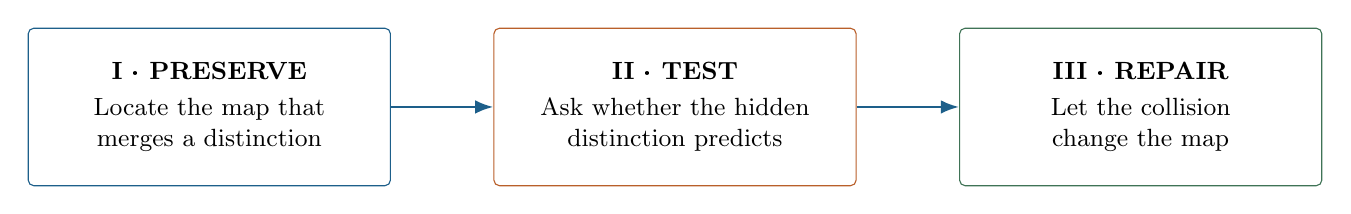
\begin{tikzpicture}[
  node distance=13mm,
  every node/.style={font=\small,align=center},
  box/.style={draw=vdink,rounded corners=2pt,minimum height=20mm,minimum width=46mm,fill=white},
  arrow/.style={-{Latex[length=2.3mm]},line width=0.9pt,color=vdblue}
]
\node[box,draw=vdblue] (one) {\textbf{I · PRESERVE}\\[2pt]Locate the map that\\merges a distinction};
\node[box,draw=vdorange,right=of one] (two) {\textbf{II · TEST}\\[2pt]Ask whether the hidden\\distinction predicts};
\node[box,draw=vdgreen,right=of two] (three) {\textbf{III · REPAIR}\\[2pt]Let the collision\\change the map};
\draw[arrow] (one) -- (two);
\draw[arrow] (two) -- (three);
\end{tikzpicture}
\end{center}

\vspace{0.42in}
The trilogy begins by separating exact state, evolution, observation, numerical access, and boundary operations. It then asks whether distinctions hidden inside a representation fibre can change a future record. Finally, it makes the representation adaptive: a meaningful collision becomes a counterexample, a typed invariant program is synthesized, and the candidate is appended before a new audit.

The result is a single progression from provenance to predictive sufficiency to constructive repair. Each paper preserves its own assumptions, claim ledger, and evidence boundary.

\vfill
\begin{center}
{\small\color{vdgray}
\textbf{Preserve the distinction.}\quad
\textbf{Test whether it matters.}\quad
\textbf{Repair the map when it fails.}}
\end{center}
\vspace{0.28in}
\clearpage

\end{document}
